% !TEX TS-program = pdflatexmk
\documentclass[11pt]{article}

\usepackage[margin=1in]{geometry}\headsep = 0.2 in
%\parskip = 0.2in
%\parindent = 0.0in

\usepackage{amsmath,amssymb,latexsym,graphicx,amsthm,enumerate}
\usepackage{palatino, url, multicol,tikz}
\newtheorem{theorem}{Theorem}
\newtheorem{corollary}[theorem]{Corollary}
\newtheorem{conjecture}[theorem]{Conjecture}
\newtheorem{lemma}[theorem]{Lemma}
\newtheorem{proposition}[theorem]{Proposition}
\newtheorem{definition}[theorem]{Definition}
\newtheorem{example}[theorem]{Example}
\newtheorem{axiom}{Axiom}
\theoremstyle{remark}
\newtheorem{remark}{Remark}
\newtheorem{exercise}{Exercise}%[section]
\def\RR{{\mathbb R}}
\def\NN{{\mathbb N}}
\def\ZZ{{\mathbb Z}}
\def\QQ{{\mathbb Q}}
\def\CC{{\mathbb C}}
\def\bc{\begin{center}}
\def\ec{\end{center}}
\def\be{\begin{enumerate}}
\def\ee{\end{enumerate}}
\def\bi{\begin{itemize}}
\def\ei{\end{itemize}}
\def\bs{\begin{slide}}
\def\es{\end{slide}}
%\def\bx{\begin{exercise}}
\newcommand{\bx}[1]{\begin{exercise}({#1} pts.)}
\def\ex{\end{exercise}}
\def\t{\times}
%\def\[{\left[}
%\def\]{\right]}
%\def\({\left(}
%\def\){\right)}
\newcommand{\ol}[1]{\overline{#1}}
\newcommand{\oimp}[1]{\overset{#1}{\Longleftrightarrow}}
\newcommand{\bv}[1]{\ensuremath{ \mathbf{\vec{#1}}} }
\renewcommand{\d}{\displaystyle}
\newcommand{\bcd}{\boldsymbol{\cdot}}

\begin{document}
{\bf Math 253 Calculus III Fall 2018 \hfill Quiz \# 1,  5 Sept 2018 }\\
\\
{\bf Name: \rule{3.5in}{1pt}}\\
\\
\noindent There are 20 points possible on this quiz. This is a closed
book quiz and closed note quiz. Calculators are not allowed. If you have any questions, please
raise your hand.

\begin{enumerate}
\item (2 points each) Use vectors $\vec{a}= 4 \vec{i} - 3 \vec{j} + \vec{k}$ and $\vec{b}= - \vec{i} +6 \vec{k}$ answer the questions below.
\begin{enumerate}
\item Find $\vert \vec{a} \vert$ \\
\vfill

\item Find $\vec{a} -3\vec{b}$ \\
\vfill

\item Find $\vec{a} \bcd \vec{b}$\\
\vfill

\item Find a \textbf{unit} vector, $\vec{u},$ in the direction \emph{opposite} vector $\vec{a}.$\\
\vfill

\item Find a vector, $\vec{w},$ of length 5 in the direction of vector $\vec{b}.$\\
\vfill

\item Determine if vector $\vec{c}= \langle 2,4,-4\rangle$ is orthogonal to vector $\vec{a}.$ You must show your work to receive credit.\\
\vfill

\item Find the scalar projection of $\vec{b}$ onto $\vec{a}.$\\
\vfill

\item Find the vector projection of $\vec{b}$ onto $\vec{a}.$\\
\vfill

\end{enumerate}
\newpage
\item (2 points each) Let vectors $\vec{u}$ and $\vec{v}$ be graphed below.\\
\begin{center}
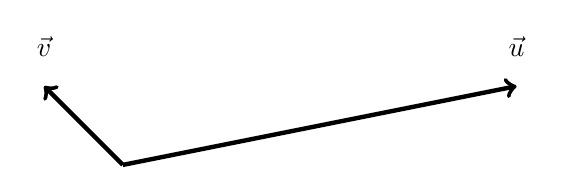
\begin{tikzpicture}
\draw[ultra thick, ->] (0,0) -- (5,1);
\draw[ultra thick, ->] (0,0) -- (-1,1);
\node at (5,1.5){$\vec{u}$};
\node at (-1,1.5){$\vec{v}$};
\end{tikzpicture}
\end{center}
\vspace{2in}

\begin{enumerate}
\item In the drawing above, sketch the vector projection of $\vec{v}$ onto $\vec{u}.$  Clearly indicate your answer.\\

\item Would the scalar projection of $\vec{v}$ onto $\vec{u}$  be positive, negative or zero? Explain your answer.\\
\end{enumerate}
\end{enumerate}
\end{document}